\section{Limitations}
\begin{table}[htbp]
  \centering
  \caption{Overview of capacitive proximity sensing limitations}
    \begin{tabular}{p{4cm}p{6cm}}
    \toprule
    \textbf{Name} & \textbf{Examples} \\
    \midrule
    \textbf{Environmental influence} & Static electric fields, dynamic electric fields, temperature, humidity, conductive objects \\
    \textbf{Physical range} & Small differences in capacitance, reduction due to influences, physical limitations \\
    \textbf{Object detection} & Small number of data points, a priori knowledge \\
    \bottomrule
    \end{tabular}%
  \label{tab:cap_limitations}%
\end{table}%

Despite the potential benefits that have been outlined in the previous section, capacitive proximity sensors have a number of limitations that may hinder several applications. 
Similar to the benefits I am putting these into three different groups that are outlined in Table \ref{tab:cap_limitations}. Environmental influences have been briefly mentioned throughout this work and have to be considered in any setup. The physical range limits the object detection to a low distance from the sensing electrode. The objection detection similarly suffers from the physical limitations of electric field sensing. These three groups will be detailed in the following paragraphs. 
\subsection{Environmental Influence}
One of the main limitations of capacitive proximity sensors is their sensitivity towards environmental influences. Any factor that modifies an electric field will also affect the measurement of a capacitive sensor. The current environmental parameters, like temperature and humidity are having a considerable effect on the atmosphere in which the electric field propagates. However, those changes are usually over a longer period of time and can be compensated using a factor for drift, as described in the previous sections about noise reduction. While the frequency range in which the sensors are operating is usually not in an interval that disturbs other electronic systems, there are some potential disturbing electromagnetic fields present in the environment. The most common sources of electromagnetic fields in the environment are power supplies (50-60 Hz) terrestrial radio in a frequency range of (150 kHz to 100 MHz), mobile phone communication (870-970 MHz and 1700-1900 MHz), as well as WiFi (2,4GHz and 5GHz). While in theory there is some potential interference with the terrestrial radio spectrum, the effect is fairly small and can be covered by choosing intermediate frequency intervals. Thus it is feasible to use capacitive sensing even in environments, where non-disturbance is a main requirement. The main source of disturbance occurring in our evaluations, was the influence of very close electromagnetic sources and disturbing signals within the power grid. One example for a disturbing source was a plasma TV installed in our Living Lab. When turned on the CapFloor prototype (\ref{ch:prot_capfloor}) that was installed below it suffered from severe noise, preventing any successful tracking of persons. The culprit are high frequency internal power supplies that drive the plasma cells. Newer TVs are using different internal electronics that significantly reduce the emitted electric field. Another disturbing factor can be created by faulty power supplies that are attached to the grid and produce frequency noise. As this noise typically operates in a limited frequency range, it is possible to use frequency domain filtering that attenuates these bands. Thus, it should be attempted to apply capacitive proximity sensing in an environment that adheres to all relevant standards regarding electromagnetic compliance. Additionally, the systems should be designed in a way that reduces potential external influences, e.g. by using internal power supplies that are stabilized and applying shielding where necessary. 
 
An additional issue might arise when placing sensors close to each other. The created electric fields may disturb the measurement if some electrodes are charged and create fields to adjacent electrodes while they are discharged for measurement. This is particularly challenging, when a larger number of sensors is involved. Here, this is the case for the CapFloor (\ref{ch:prot_capfloor}) and CapTap (\ref{ch:prot_captap}) prototypes. In the case of CapTap specific charge-discharge cycles for the electrodes are used that ensure that adjacent sensors are not interfering with each other. Similarly the CapFloor attempts to control the sensors in a way that prevents interference, taking into account the geometric layout and the position of the electrodes within the area. Both methods are a form of multiplexing that is based on time (TDMA).Other options include a variety of different multiplexing methods, such as the previously mentioned frequency method of Honeyfish (\ref{ch:prot_otherprot}). Code division multiplex is a last class of multiplexing methods that relies on the modification of the signal. This was employed by the presented capacitive sensor of Rob MacLachlan \cite{MacLachlan2004}. This can result in very precise measurement but requires specialized hardware. Thus it was not used in any of the developed prototypes.

A major challenge is dealing with conductive objects that are permanently placed in the immediate sensing environment. It is difficult to distinguish the object we want to detect from a disturbing object, if their influence on the electric field is similar. Long term data analysis may help in performing a successful detection. The CapTap prototype, as a regular living room table, should not fail when disturbing objects, such as glasses full of water (\ref{ch:prot_captap}). This can be achieved by performing a feature analysis that detects the typical response of the disturbing object and performs a recalibration that takes the object into account. 

The CapFloor prototype is affected by environmental influences the most, given the small size of the electrodes relative to the interaction area and the changing environment on top of the floor (\ref{ch:prot_capfloor}). We are using a strong noise reduction algorithm and drift compensation to create a more stable result that however causes a reduction of the detection range.
\subsection{Physical Range}
\begin{minipage}{\linewidth}
\centering
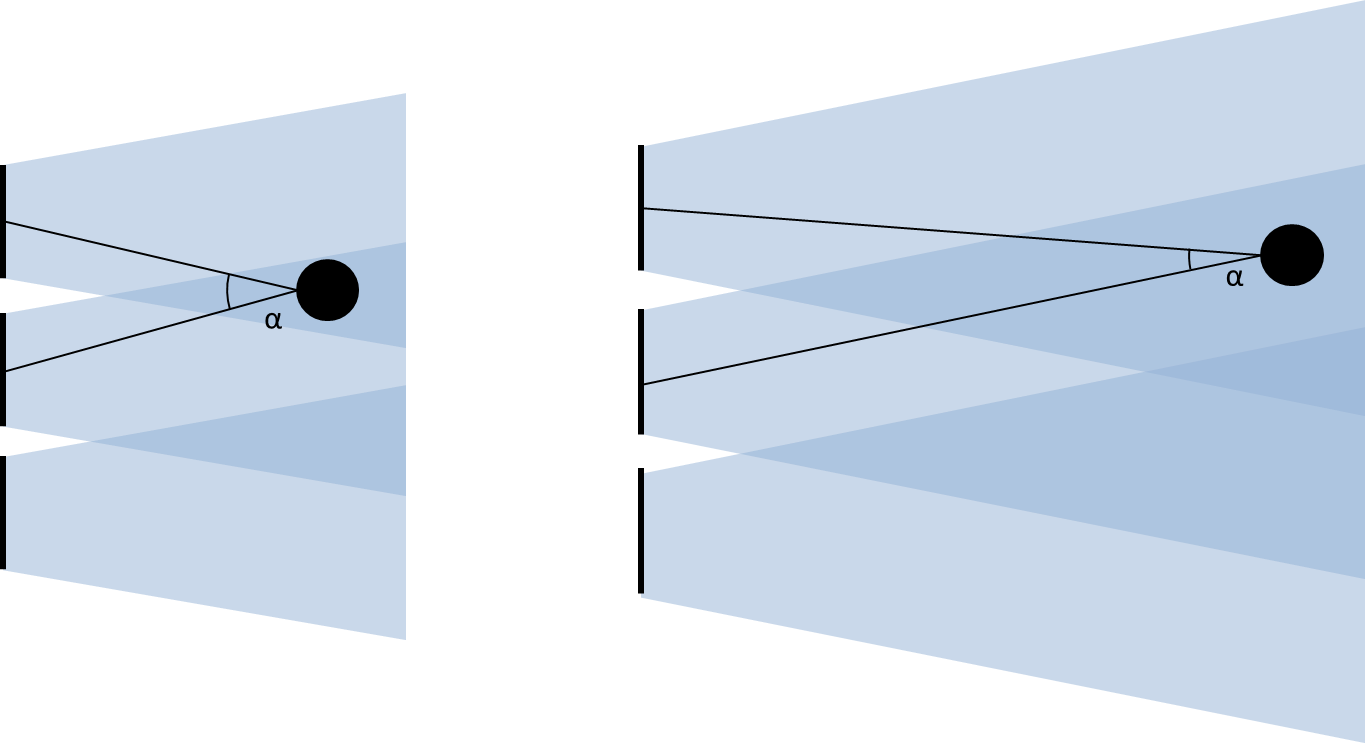
\includegraphics[width=0.8\textwidth]{images/limit_distance}
\captionof{figure}{Reduced angular resolution on smaller, distant objects}
\label{fig:disc_ang_resolution}
\end{minipage}

The physical range of the generated electric field is one of the main limiting factors of capacitive proximity sensing. In order to detect objects that are further away, we have to increase the electric field strength sufficiently. This is easier the larger the electrode is, as its potential capacitance is higher. However, this also leads to distant objects having an ever smaller influence on the overall capacitance, and we need more precise measurement circuits and longer measurement times to improve the signal-to-noise ratio. Additionally, looking at smaller objects the angular resolution will decrease as shown in Figure \ref{fig:disc_ang_resolution}. This makes it more difficult to get a precise localization as the immanent noise leads to an angular error. While this can be compensated using more sensors, the far distance would require us to use large electrodes that have to be placed further apart resulting in a huge area that would have to be equipped with sensor electrodes. The Capacitive Chair prototype uses large electrodes that allow us to detect the presence of a person at distances of around 50-60 cm (\ref{ch:prot_capchair}). It is designed to detect whole body parts and thus does not need any fine resolution. The Active Armrest on the other hand has the finger interaction array comprised of small electrodes that have a detection limit of approximately 15 cm (\ref{ch:prot_armrest}). Yet, it is able to detect fine movements and precise locations of the fingers within this range.

In general the achievable resolution is not comparable to vision based system and has to be taken into consideration when designing the specific application. A balance between electrode size, physical range and achievable resolution has to be found. The MagicBox size does not allow an integration of very large electrodes (\ref{ch:prot_magicbox}). Instead, we are optimizing the available space in order to achieve a detection that lets us detect hands in a distance of approximately 30 cm and allows reliable tracking in distances between 15 and 20 cm. The system with the lowest detection distance is the CapFloor prototype (\ref{ch:prot_capfloor}). The long wire electrodes are not particularly suited for achieving a good resolution and are prone to interference. However, they are suitable for this specific purpose and objects at a proximity of 10 cm can still be detected. 
\subsection{Object Detection}
\begin{minipage}{\linewidth}
\centering
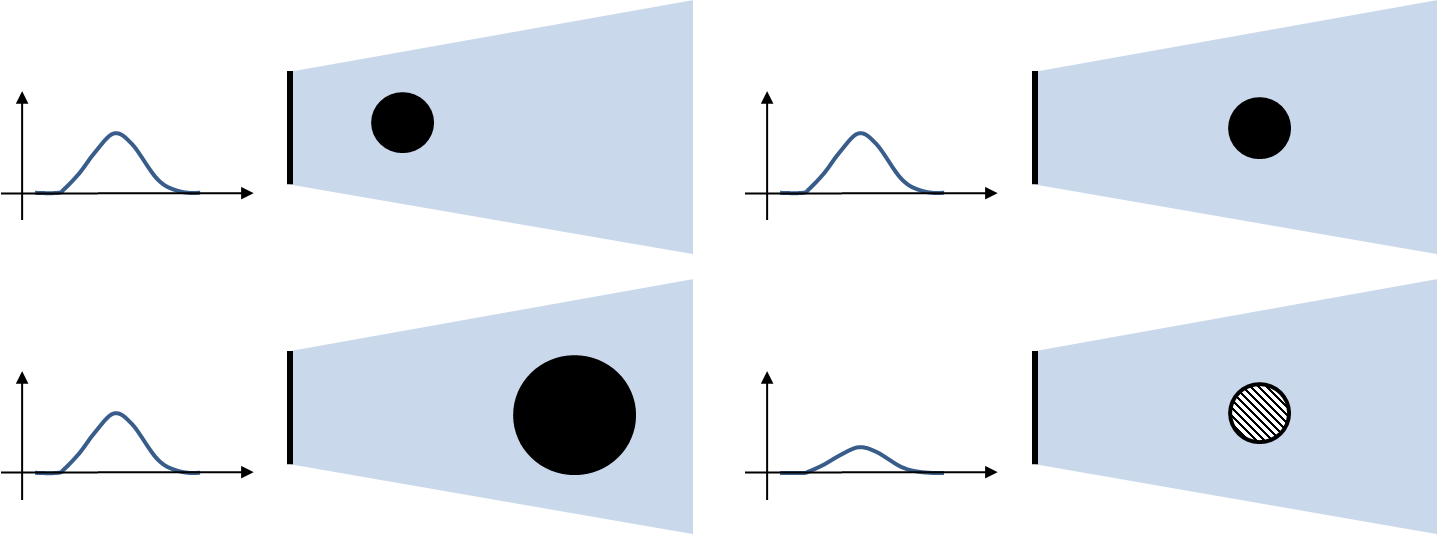
\includegraphics[width=0.8\textwidth]{images/limit_detection}
\captionof{figure}{Same response to differently sized objects (left), different response to varying materials (right)}
\label{fig:disc_obj_detection}
\end{minipage}

Object detection using capacitive sensors can be partially compared to object detection using camera systems, with a single sensor being equivalent to a single photo sensor. Smith et al. propose that loading mode measurements resemble light captured by a camera without a lens as only one part of the electric system is constrained \cite{smith1998electric}. The light intensity measure is comparable to field intensity and likewise it is not possible to distinguish if the measurement is caused by a weak source in close proximity or a strong source at a further distance. As a practical example the capacitive sensor is not able to decide if one hand is close to the sensor or two hands are a bit further away. This effect makes it challenging to provide object detection and we usually have to combine the information from various sensors to get a good idea about object shape and size. The CapTap prototype is able to detect two hands by combining the information of 24 sensors and additionally uses an analysis of the arm posture in the detection area (\ref{ch:prot_capfloor}). Due to the presented challenges in physical range and electrode size, capacitive proximity sensing systems do not have the same level of scalability as opposed to cameras, where millions of photo sensors can be placed in very small areas. Touch screens show that capacitive sensing technology has a very high resolution in near ranges. However, this is can't be translated to similar resolution in further distances.

Additionally, the effect of an object on the electric field is not always closely correlated to the object dimensions, but instead based on conductivity, material and other factors. We may get the same response to different objects at different distances or get a varying on similarly sized objects made of different materials, as shown in Figure \ref{fig:disc_obj_detection}. In the presented application scenarios exclusively parts of the human body are tracked. Mostly, there is also an assumption that no other objects should be used. The CapTap will have to identify potential foreign objects from the hands of the user (\ref{ch:prot_captap}). In this case the specific capacitance profile of objects at close proximity can be used, similar to the capacitance tags presented by SmartSkin \cite{rekimoto2002smartskin}. The Active Armrest has gestures for one and two fingers that are distinguished using a simple threshold (\ref{ch:prot_armrest}). If another object is entering the field or the person is having a strongly different finger size, the system will fail to properly differentiate gestures. Accordingly some other compensation methods should be used.

